\graphicspath{{./Komora/images/}}

\chapter{Program komputera komory środowiskowej}

Komora środowiskowa jest częścią urządzenia, w której zachodzi wzrost badanej struktury biologicznej. Kluczowe dla jej wzrostu jest zachowanie pewnych cech takich jak odpowiednia ilość dostępnej wody w jej podłożu wzrostowym lub odpowiednie oświetlenie. Oprócz tego przydatne może okazać się śledzenie parametrów takich jak temperatura. Komora środowiskowa jest też miejscem docelowym, gdzie działanie grawitacji jest eliminowane poprzez klinorotację. Muszą się więc znajdować również w niej czujniki, które jakość symulowanej mikrograwitacji będą monitorować.

\section{Platforma}

Wybór platformy komputera komory środowiskowej został dokonany na etapie tworzenia projektu urządzenia. Wybrany został komputer Raspberry Pi Zero ze względu na niski pobór energii, co było kluczowe ze względu na ograniczenia prądowe złącz ślizgowych oraz generowane przez komputer pola magnetyczne, które w przypadku wyższych mocy mogą zaburzyć jednorodność pola. Posiada on również wbudowany moduł Wi-Fi za pomocą którego zrealizowano połączenie bezprzewodowe. Umożliwia to także zdalną obsługę komputera poprzez standard SSH (ang. \angver{Secure Shell}) w momencie gdy nastąpi awaria oprogramowania.\linebreak Ze względu na konieczność obsłużenia kamer oraz analogowego czujnika wilgotności podłoża, komputer wyposażono w dodatkowe nakładki, które zwiększają ilość dostępnych portów USB oraz dodają konwerter analogowo-cyfrowy (ang. \angver{Analog to Digital Converter}, ADC) do magistrali I$^2$C. Na komputerze zainstalowano system operacyjny Raspbian Lite, który nie posiada graficznego interfejsu użytkownika\linebreak w związku z czym ogranicza zużycie jego zasobów.

\section{Rola programu}

Główną rolą programu jest odczytywanie wartości zbieranych przez szereg czujników, a następnie przekazywanie ich do głównej aplikacji w celu wyświetlenia oraz zapisania w pliku. Oprócz tego program kontroluje oświetlacz komory środowiskowej poprzez regulację sygnału PWM podawanego na jego układ sterujący. Program kontroluje dwie sekcje oświetlacza o osobnych sygnałach PWM oraz dodatkowe diody białe służące do doświetlenia układu w momencie wykonywania zdjęcia.\linebreak W celu wykonania zdjęć do komputera podłączone zostaną dwie kamery USB, które będą wykonywać zdjęcia zgodnie z poleceniami generowanymi w programie. Program oblicza również na bieżąco jakość uzyskanego stanu mikrograwitacji.

\section{Komunikacja bezprzewodowa}

Komunikacja z poziomu komputera komory została w znacznym stopniu zautomatyzowana. Użytkownik musi jedynie zawrzeć spodziewany adres serwera TCP na którym komora będzie go szukać, w pliku konfiguracyjnym. W momencie kiedy taki serwer zostanie uruchomiony z poziomu aplikacj, komputer komory automatycznie go wykryje i zacznie wymieniać informacje. Kiedy serwer nie został uruchomiony, komora ponawia próbę połączenia co \SI{5}{s}, aż do momentu kiedy ta operacja zakończy się powodzeniem. Jeśli takie połączenie zostaje nagle zerwane, komputer komory powraca do stanu próby połączenia.
\begin{lstlisting}[language=Python,caption={Obsługa połączenia z serwerem TCP.}]
while True:
	while True:
		with socket.socket(socket.AF_INET, socket.SOCK_STREAM) as sc:
		
			sc.settimeout(5)
			try:
				print(f"Attempting connection to {address}")
				sc.connect((address, port))
			except socket.timeout:
				print("Connection timed out.")
				break
			except ConnectionRefusedError:
				index = 0
				means = [0, 0, 0]  # Resetting the gravity averages.
				saturation_measurement_scheduled = False
				print("Connection refused, reconnection attempt in 5s.")
				time.sleep(5)
				break  # Here interrupt the inner forever loop and continue to watch for the connection.
\end{lstlisting}

Kiedy połączenie zostanie pomyślnie nawiązane, rozpoczyna się proces wymiany informacji. Na Rys. \ref{fig:ramka danych} przedstawiono schematycznie w jaki sposób zbudowane są ramki danych wymieniane pomiędzy urządzeniami. Pierwsza część ramki składa się z nagłówka o długości \SI{10}{B}, który zawiera informację o tym ile kolejnych bajtów należy odebrać, aby skompletować wiadomość. Jeśli dana paczka została odebrana przez serwer, odsyła on informację o tym czy należy zauktualizować warunki oświetleniowe, co jest determinowane poprzez akcję użytkownika. Jeśli operator nie zmienił ustawień oświetlenia od poprzedniej wymiany danych, to wysyłany jest jedynie komunikat sygnalizujący zachowanie poprzedniego ustawienia. Cykl ten powtarza się tak długo, jak istnieje połączenie pomiędzy komorą środowiskową a rdzeniem systemu kontroli.


\begin{figure}[h]
	\centering
	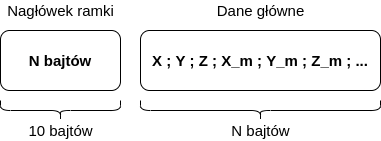
\includegraphics[scale=.5]{ramka}
	\caption{Schemat wiadomości wymienianych pomiędzy urządzeniami. Źródło: [opracowanie własne].} 
	\label{fig:ramka danych}
\end{figure}


\section{Czujniki i kamery}

W celach uproszczenia starano się dobrać czujniki tak, aby wszystkie mogły zostać obsłużone przez taki sam interfejs. Do tego celu wybrano magistralę I$^2$C ze względu na jej dużą popularność oraz dostępność różnego rodzaju czujników. Na tę samą magistralę znalezniono również konwerter analogowo-cyfrowy, którego nie posiada domyślnie wybrana platforma. Oprócz czujników komputer obsługuje również dwie kamery, aby uwiecznić postęp wzrostu struktury. Poniżej umieszczono listę modeli wybranych czujników oraz kamer.
\begin{itemize}
	\item Akcelerometr LIS3DH, magistrala I$^2$C
	\item Termometr MCP9808, magistrala I$^2$C
	\item Konwerter analogowo-cyfrowy ADS1115, magistrala I$^2$C
	\item Moduł kamery OV5648, port USB
	
\end{itemize}

Dla czujników przygotowany został osobny moduł \textbf{sensors.py}, który zawiera definicje klas odpowiedzialnych za tworzenie interfejsu między nimi a komputerem komory środowiskowej. Jako, że wszystkie obiekty czujników muszą posiadać metody odpowiedzialne za wysyłanie do nich danych lub ich odbieranie, zostały one oparte o dziedziczenie z abstrakcyjnej klasy bazowej (ang. \angver{abstract base class}, ABC). Oznacza to, iż dzielą one metody o takiej samej nazwie, które docelowo przeznaczone są do tych samych celów, mimo tego iż mogą różnić się zawartością.
\begin{lstlisting}[language=Python, caption={Abstrakcyjna klasa bazowa czujników.}]
class I2CSensor(ABC):

	def __init__(self, address, bus):
		self.address = address
		self.bus = bus
	
	@abstractmethod
	def read(self, *args, **kwargs):
		pass
	
	@abstractmethod
	def enable(self, *args, **kwargs):
		pass
	
	@staticmethod
	@abstractmethod
	def fake_read():
		pass	
\end{lstlisting}
Metody w jakie wyposażono obiekty czujników to wspólny konstruktor \textbf{\_\_init\_\_}, który inicjalizuje obiekt przy okazji przypisując mu otwartą magistralę oraz adres, \textbf{read} zwracającą odczytaną wartość z czujnika, \textbf{enable}, która dokonuje wszystkich operacji koniecznych do poprawnego działania czujnika oraz \textbf{fake\_read}, która emuluje odczyt z czujnika bez konieczności jego podłączenia, co było pomocne\linebreak w czasie rozwoju programu. Po tak przygotowanej klasie bazowej dziedziczą klasy reprezentujące już konkretne modele czujników, ze względu na różny algorytm odbioru z nich informacji.
\begin{lstlisting}[language=Python, caption={Przykładowa klasa czujnika.}]
class ADS1115ADC(I2CSensor):
	
	__CONVERSION_REG = 0x00
	__CONFIG_REG = 0x01
	__LO_THRESH_REG = 0x02
	__HU_THRESH_REG = 0x03
	
	def read(self, channel):
		# Read channel voltage in reference to ground. ADS1115 also has a differential measuring mode, which
		# has been omitted, but would be trivial to implement.
		
		ls_byte = 0b11100011  # Comparators disabled, 860SPS data rate
		ms_byte = 0b0011 + ((channel + 4) << 4) + 128  # Amplifier gain set to 1, start single conversion, pick channel.
		self.bus.write_i2c_block_data(self.address, ADS1115ADC.__CONFIG_REG, [ms_byte, ls_byte])
		while self.converting_status():
			pass
		data = self.bus.read_i2c_block_data(self.address,ADS1115ADC.__CONVERSION_REG,2)
		reading = (data[0] << 8) + data[1]
		
		return reading
	
	def enable(self):
		pass
	
	@staticmethod
	def fake_read() -> float:
	
		base_read = 50
		
		return float(np.random.normal(base_read, 10, 1))
	
	def converting_status(self):
	
		config = self.bus.read_i2c_block_data(self.address, ADS1115ADC.__CONFIG_REG, 2)
		
		if config[1] >= 128:
			return False
		else:
			return True
\end{lstlisting}

Kamery również obsługiwane są z poziomu programu poprzez wywoływanie poleceń w powłoce systemowej za pomocą biblioteki \textbf{subprocess}. W tym celu przygotowano prosty skrypt \textbf{take\_pic.sh}, który wykonuje zdjęcia za pomocą obu kamer przy użyciu interfejsu Video4Linux. Konieczne jest, aby obie kamery posiadały odpowiednie nazwy adapterów portu a, konkretnie \textbf{/dev/videoCam0} oraz \textbf{/dev/videoCam1}. Uzyskiwane jest to za pomocą pliku reguł \textbf{99-name-cameras.rules}, który rozpoznaje unikatowe dla kamer cechy i tworzy odpowiednie dowiązania symboliczne. Plik ten został również umieszczony w repozytorium projektu i należy umieścić go w katalogu \textbf{/etc/udev/rules.d/} w systemie plików komputera komory środowiskowej. Należy zaznaczyć iż numery umieszczone w pliku reguł odpowiadają konkretnym egzamplarzom kamer, a więc jeśli zostaną one zamienione, należy ów kod również zamienić.
\begin{lstlisting}[caption={Plik reguł \textbf{99-name-cameras.rules}.}]
SUBSYSTEM=="video4linux", ENV{ID_REVISION}=="5131",SYMLINK+="videoCam0"
SUBSYSTEM=="video4linux", ENV{ID_REVISION}=="5127",SYMLINK+="videoCam1"
\end{lstlisting}

Na etapie projektu przetestowano kilka dostępnych na rynku czujników wilgotności gleby. Każdy z nich charakteryzował się szybkim postępem korozji elementów wystawionych na działanie wody. Stworzono więc autorski czujnik składający się z dwóch igieł wykonanych ze stali nierdzewnej. Pomiar wilgotności odbywa się poprzez pomiar napięcia układu, w którym układ igieł wbitych w podłoże wzrostowe działa jak rezystor o zmiennym oporze. Aby ograniczyć korozję czujnika do minimum, zasilanie układu jest włączane jedynie na czas pomiaru, trwający 3s. Na Rys. \ref{fig:czujnik wilg} przedstawiono głowicę wykonanego czujnika wilgotności. Napięcie z układu mierzone jest poprzez dołączony do komputera przetwornik analogowo-cyfrowy. Na Rys. \ref{fig:czujnik wilg sch} widoczny jest prosty schemat elektryczny obwodu czujnika. Zasilanie doprowadzone jest do układu poprzez tranzystor (w tym wypadku jest to fototranzystor zawarty w transoptorze), sterowany z poziomu programu komputera komory środowiskowej. Aby poprawnie interpretować poziomy napięć, konieczny jest pierwszy pomiar napięcia dla głowicy czujnika zanurzonej w wodzie z docelowym stężeniem substancji odżywczych. Dalsze pomiary są następnie przeprowadzane w odniesieniu do tak przygotowanej referencji.

\begin{figure}[h]
	\centering
	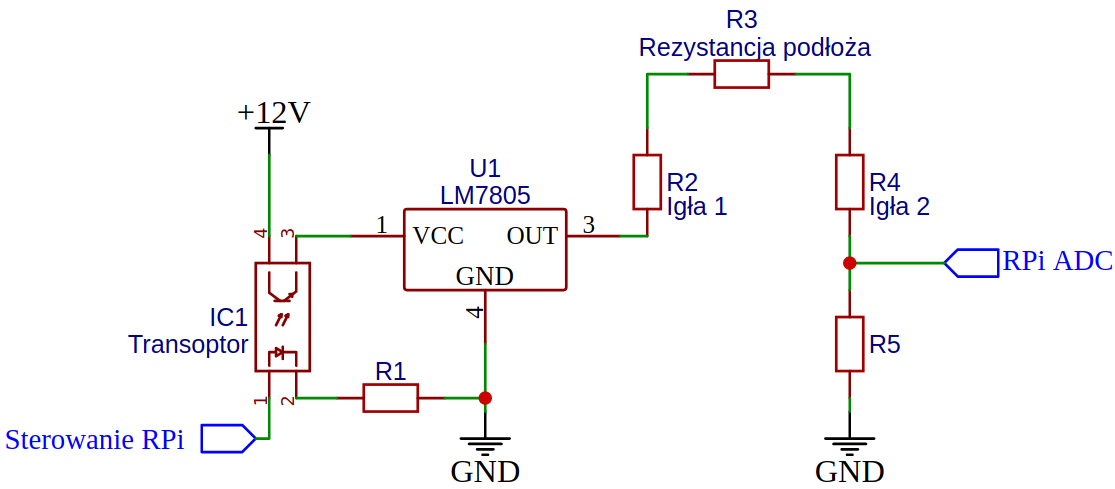
\includegraphics[scale=.4]{schemat_wilg}
	\caption{Schemat elektryczny obwodu czujnika. Źródło: [opracowanie własne].} 
	\label{fig:czujnik wilg sch}
\end{figure}

\begin{figure}[h]
	\centering
	\setlength{\fboxsep}{0pt}
	\setlength{\fboxrule}{1pt}
	\fbox{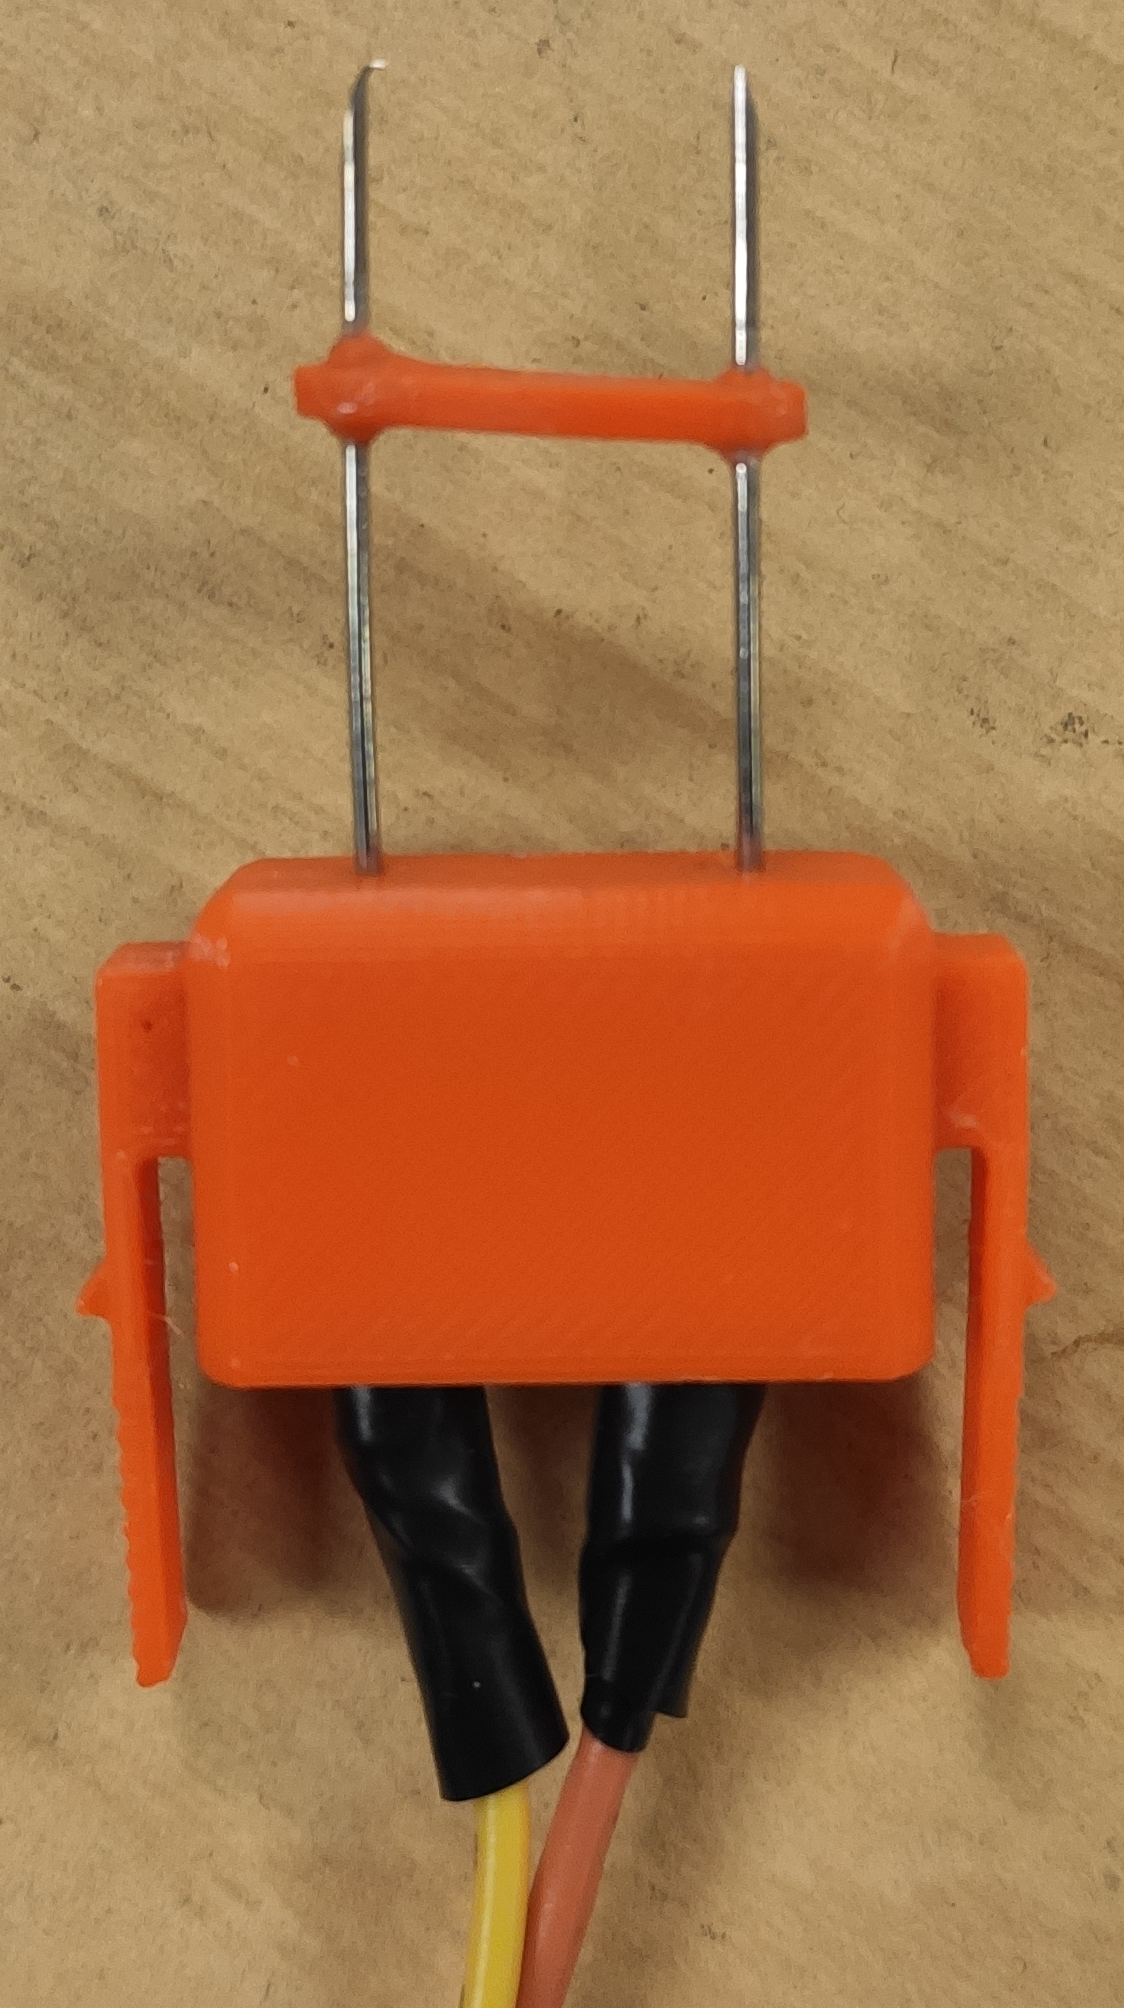
\includegraphics[scale=.15,angle=90]{czujnik_wilg}}
	\caption{Wykonana głowica czujnika wilgotności podłoża. Źródło: [opracowanie własne].} 
	\label{fig:czujnik wilg}
\end{figure}